\section{Architektura aplikace}\label{analyza-architektura}

Jako doporučenou architekturu aplikací pro platformu iOS (konkrétně iPhone a iPad) uvádí Apple Model-View-Controller (zkráceně \acrshort{mvc}).
Přestože je \acrshort{mvc} pro vývoj aplikací nejpopulárnější, rozhodl jsem před začátkem implementace prozkoumat i jiné existující architektury.
Z alternativních architektur jsem nakonec zvolil Model-View-ViewModel, kterou porovnám s doporučeným \acrshort{mvc}.
V závislosti na výsledku porovnání zvolím ideální architekturu pro svou aplikaci.

\subsection{\acrshort{mvc}: Model-View-Controller}\label{analyza-mvc}
Tato architektura rozděluje aplikaci do tří vrstev: Model, View a Controller.

\subsubsection*{Popis architektury}

\begin{figure}\centering
	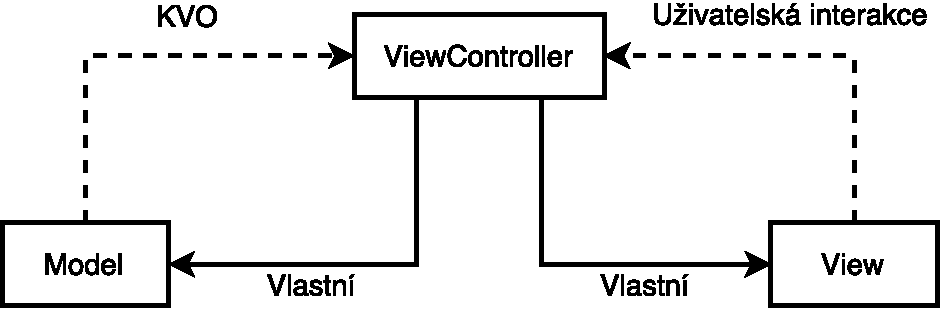
\includegraphics[width=0.75\textwidth]{assets/analysis-mvc-architecture.pdf}
	\caption{Architektura MVC}\label{fig:architektura-mvc}
\end{figure}

\begin{description}
  \item[Model] reprezentuje perzistentní objekty, které aplikace využívá pro vnitřní logiku a prezentaci dat uživateli.
  Každý modelový objekt může být v relaci s libovolným počtem jiných modelových objektů.
  Tato vrstva je často reprezentována databází, příkladem mohou být databáze CoreData, Realm nebo SQLite.
  Ukázka \ref{code:mvc-model} prezentuje možnou podobu modelového objektu.
  \swiftcode{code:mvc-model}{Modelový objekt v architektuře \acrshort{mvc}}{assets/code/mvc-model.swift}

  \item[View] je datový objekt viditelný uživatelem. View obsahuje logiku pro vykreslení a interakci s uživatelem.
  Přestože se View standardně používá pro zobrazení modelových objektů nebo jejich úpravu, jsou od sebe tyto vrstvy striktně odstíněny.
  Na platformě iOS tuto vrstvu reprezentuje framework UIKit vytvořený Applem.
  Ukázkový kód \ref{code:mvc-view} zobrazuje možnou implementaci View.

  \item[Controller] je aplikační vrstva, která na základě vstupů z View aktualizuje a mění Model nebo překresluje View v případě, že zobrazovaná data už nejsou aktuální.
  Jedním z úkolů Controlleru je striktně zamezit přímé interakci mezi View a Modelem.
  Toto oddělení je zavedeno proto, aby View nemuselo znát konkrétní strukturu Modelu a aby Model nemusel obsahovat logiku formátování dat (cena, čas, ...) pro vykreslení.
  Dále se stará o navigaci mezi obrazovkami, síťování a interakci s uživatelem.
  Při rozdělení do obrazovek platí pravidlo, že jeden Controller obsluhuje jedno nebo více View.
  Ke korektnímu vykreslení View využívá libovoné množství modelových objektů.
  O jednu obrazovku se typicky stará právě jeden Controller, je ale možné jich použít více.
  Zjednodušenou implementaci lze vidět v ukázce \ref{code:mvc-view-controller}.
\end{description}

Z tohoto shrnutí vyplývá, že Controller je velmi blízce spjat s View. Toto propojení reprezentuje obrázek \ref{fig:massive-mvc}.

\subsubsection*{Modelový příklad použití}

Pro možné porovnání architektury jsem připravil scénář stažení libovolných dat na základě požadavku uživatele.
V \acrshort{mvc} by se architektura chovala takto:

\begin{itemize}
  \item Uživatel v aplikaci klikne na tlačítko \uv{Stáhnout data}.
  \item Tuto interakci odchytí View a upozorní Controller.
  \item Controller na základě upozornění stáhne data a předá je Modelu k uložení.
  \item Model ukládá data a notifikuje Controller o změně.
  \item Controller aktualizuje View.
  \item Nastane-li během stahování chyba, Controller vytváří nové View a chybu prezentuje uživateli.
\end{itemize}

\swiftcode{code:mvc-view}{View v architektuře \acrshort{mvc}}{assets/code/mvc-view.swift}

\subsubsection*{Shrnutí}

Shrneme-li vlastnosti vrstev, jejich klíčové role jsou:

\begin{itemize}
  \item Model udává, jakým způsobem jsou data uložena,
  \item View se stará o správné vykreslení předformátovaných dat,
  \item Controller se stará o ostatní logiku.
\end{itemize}

\swiftcode{code:mvc-view-controller}{ViewController v architektuře \acrshort{mvc}}{assets/code/mvc-view-controller.swift}

Pro zmíněné notifikace nabízí Apple řešení pomocí Delegate pattern.
Controller musí naimplementovat specifické rozhraní, čímž se stane delegátem.
Jako delegát se pak může zaregistrovat na notifikace obejktů, jejichž rozhraní implementoval.

\acrshort{mvc} je v době psaní této práce nejpoužívanější architekturou a to především díky své jednoduchosti.
Při tvorbě větších aplikací ale nemusí být vhodné.
Controller se při nestandradním grafickém návrhu může stát velmi složitým, což výrazně snižuje jeho čitelnost a testovatelnost.
Z tohoto důvodu se \acrshort{mvc} často přezdívá \uv{Massive View Controller}.
Díky přímému napojení controlleru na View se při testování chování Controlleru (behavioral testing) musí využít simulátoru mobilního operačního systému a aplikaci v něm automaticky \uv{proklikat}.
To zvyšuje časovou náročnost testování, dokonce v některých případech znemožňuje testování úplně (Controlleru nezle podvrhnout mock objekty).
Tento problém se snaží řešit architektura \acrshort{mvvm} od společnosti Microsoft.

\begin{figure}\centering
	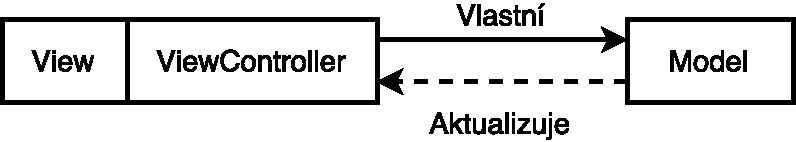
\includegraphics[width=0.75\textwidth]{assets/analysis-massive-view-controller.pdf}
	\caption[Role Controlleru v MVC]{Controller spjatý s View}\label{fig:massive-mvc}
\end{figure}

\subsection{MVVM: Model-View-ViewModel}\label{analyza-mvvm}

Z důvodu nárustu nároků na mobilní aplikace se v posledních letech rozmáhá architektura \acrshort{mvvm}.
Tato architektura vychází ze zmíněného \acrshort{mvc} a jejím základním úkolem je zjednodušit Controller.

\subsubsection*{Popis architektury} \label{architektura-mvvm-popis}

Za účelem zjednodušení Controlleru se ke stávajícím třem vrstvám přidává ViewModel, který se stará o přípravu dat z Modelu pro zobrazení a také o perzistenci změn.

\begin{description}
  \item[ViewModel] je objekt vlastněný Controllerem za pomoci kompozice.
  Pro Controller připravuje naformátované výstupy a poskytuje mu rozhraní pro vstupy.
  Výstupem se rozumí veškerá data, která jsou potřebná pro sestavení View.
  To může být např. datum ve specifickém formátu, cena včetně měny nebo informace o tom, kolik řádků bude obsahovat tabulka na obrazovce.
  Oproti \acrshort{mvc} tedy perzistentní data nejsou viditelná Controlleru, ale pouze ViewModelu.
  Ten je nejdříve připraví pro zobrazení.
  Vstupem může být libovolná interakce uživatele:
  změna textu v textovém poli, stisknutí tlačítka, ale i fyzický pohyb telefonem (otočení obrazovky).
  Na základě vstupů spouští ViewModel svou vnitřní logiku a generuje výstupy.
  Jednoduchou implementaci ViewModelu bez použití vstupů lze vidět v ukázce \ref{code:mvvm-view-model}.
\end{description}

\swiftcode{code:mvvm-view-model}{ViewModel v architektuře \acrshort{mvvm}}{assets/code/mvvm-view-model.swift}

Zodpovědnost Controlleru se zavedením ViewModelu dramaticky snižuje.
V ideálním případě je Controller zodpovědný pouze za správné sestavení View a napojení zfromátovaných výstupů na něj.
Dále pak za odchycení uživatelských interakcí a jejich propagaci do ViewModelu.
Toto chování zachycuje obrázek \ref{architektura-mvvm}.

\begin{figure}\centering
	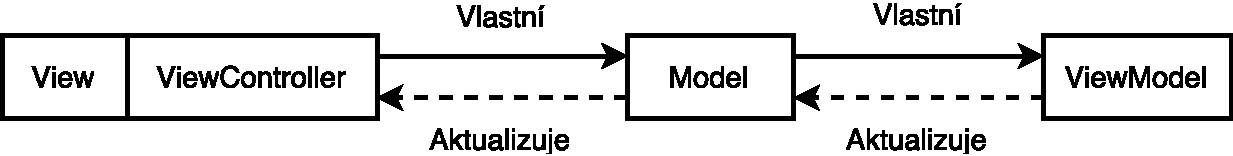
\includegraphics[width=0.9\textwidth]{assets/analysis-mvvm-architecture.pdf}
	\caption[Architektura \acrshort{mvvm}]{Architektura \acrshort{mvvm}}\label{architektura-mvvm}
\end{figure}

\subsubsection*{Modelový příklad použití} \label{architektura-mvvm-priklad}

Pro porovnání architektury s \acrshort{mvc} lze opět využít scénář pro stažení dat.
Pro tento scénář by se architektura \acrshort{mvvm} chovala následovně:
\begin{itemize}
  \item Controller napojuje výstupy ViewModelu na View a vytváří pravidla pro převod uživatelské interakce na vstupy ViewModelu.
  \item Uživatel v aplikaci klikne na tlačítko \uv{Stáhnout data}.
  \item View upozorňuje Controller na interakci uživatele, ten automaticky vytváří vstup pro ViewModel.
  \item ViewModel na základě vstupu stahuje data a předává je Modelu.
  \item Model po uložení notifikuje ViewModel, ten vytváří výstup pro Controller, který nechává překreslit View.
  \item V případě chyby vytvoří ViewModel chybový výstup, ten se pomocí Controlleru propaguje do View.
\end{itemize}

\subsubsection*{Shrnutí} \label{architektura-mvvm-shrnuti}

Vrstvy mají následující klíčové vlastnosti:
\begin{itemize}
  \item Model definuje jakým způsobem jsou data uložena a při změně notifikuje ViewModel,
  \item View vykresluje na obrazovku naformátované výstupy a upozorňuje controller při interakci uživatele,
  \item Controller sestavuje hierarchii View, napojuje zformátované výstupy ViewModelu na View a z uživatelské interakce vytváří vstupy pro ViewModel,
  \item ViewModel načítá data Modelu. Na základě vstupů z Controlleru nebo změny Modelu generuje výstupy pro Controller.
\end{itemize}

Oproti \acrshort{mvc} je na tomto příkladu vidět snížení zodpovědnosti Controlleru.
Tato zodpovědnost se přesunula do ViewModelu (viz. ukázka \ref{code:mvvm-view-controller}).
Na první pohled nemusí být tato změna opodstatněná, protože logika aplikace nezmizela, jen se přesunula.
Právě to ale umožnilo (nebo minimálně zjednodušilo) způsob, jakým lze logiku testovat.
ViewModel generuje výstupy na základě vstupů, v testech tedy lze uživatelskou interakci podvrhnout a testovat pouze výstupy (není potřeba vytvářet View ani Controller).
Dodatečně lze otestovat i uživatelské rozhraní.
Protože logika aplikace je otestována pomocí testů ViewModelu, uživatelské rozhraní už stačí otestovat např. shodou View s referenčním obrázkem.

\swiftcode{code:mvvm-view-controller}{Controller v architektuře \acrshort{mvvm}}{assets/code/mvvm-view-controller.swift}

Při pohledu na notifikace je vidět, že přibyl typ, který nebyl v \acrshort{mvc} potřeba.
Jedná se o notifikace směrem z ViewModelu ke Controlleru (ViewModel nemá referenci na Controller, nemůže ho notifikovat přímo).
Některé výstupy View Modelu je tedy potřeba sledovat v čase a na jejich změny reagovat.
Toto lze vyřešit pomocí \acrshort{kvo}, které nabízí Apple mezi standardními knihovnami.
\acrshort{kvo} umožňuje objektu zaregistrovat se na notifikace o změně stavu nějakého libovolného jiného objektu.
V případě Controlleru by se registroval na změny stavu výstupů ViewModelu.
Kdykoliv by se výstup změnil, Controller by dostal notifikaci.
Tento přístup ale není běžný pro použití s jazykem Swift.
Tento postup navíc neřeší synchronizaci vláken, z tohoto důvodu by mohlo docházet k nekonzistenci dat či neočekávanému chování.
Místo \acrshort{kvo} se nyní standardně používají reaktivní rozšíření, které popisuji v následujících kapitolách.

Přestože mnou implementovaná aplikace není v ohledu na uživatelské scénáře nijak složitá, obsahuje mnoho obrazovek.
Obrazovky jsou vysoce interaktivní a více se k jejich implementaci hodí reaktivní přístup.
